\documentclass{article}
\usepackage{graphicx} 
\usepackage{longtable}
\usepackage{hyperref} 
\usepackage{geometry} 
\usepackage{caption}
\usepackage{float}
\geometry{a4paper, margin=1in}

\title{Technical Writing Documentation: Snapchat Application}
\author{}
\date{}

\begin{document}
\newpage
\begin{center}
    {\LARGE \textbf{Technical Writing Documentation:}} \\
    \vspace{0.5cm}
    {\LARGE \textbf{Snapchat Application}}
\end{center}
\vspace{3cm}
\begin{longtable}{|p{3cm}|p{2.5cm}|p{7cm}|}
    \hline
    \textbf{ Student Name } & \textbf{ Student ID } & \textbf{ Work } \\
    \hline
    Mayar Abkar Noli & 
    444005019 &
    •Introduction section: Abstract, Survey, Existing programs \newline
    •Analysis section: All \newline
    Design section: User Interface, Data Model, Database. 
    \\
    \hline
    Ghaidaa Ibrahim Al-Sheikhi & 
        44410080 &
    • Introduction section: Background, Main Tasks, Existing programs. \newline
    •Design section: Data Model, Programing Languages \\
    \hline
    \caption{group}
    \label{tab:group}
\end{longtable}


\newpage
\tableofcontents

%\newpage
%\begin{center}
 %   \textbf{\Large Introduction}  
%\end{center}
\newpage
\section{Introduction}  

\subsection{Abstract}

This document presents an analysis of the Snapchat application, focusing on its features, design, and functionality. It examines how Snapchat has redefined social media through its ephemeral content model, allowing users to share moments that disappear after a short period. The study also compares Snapchat with other platforms, specifically Instagram and TikTok, highlighting the unique strengths and limitations of each. Functional and non-functional requirements for the app are identified, covering areas like user interaction, privacy controls, and system performance. Furthermore, the architectural design of the application, including its user interface, database is explored. This document aims to provide insights into the core aspects of Snapchat, illustrating how it maintains user engagement while addressing modern challenges in usability, privacy, and scalability.

\subsection{Background}

Online communication has become an integral part of our daily lives, as modern technology has changed the way we interact with others. Communication has evolved tremendously to include multiple platforms such as social networks, messaging apps, and forums. These means allow individuals to exchange ideas and information easily and quickly, which contributes to building social, economic and cultural relationships. Through platforms like Snapchat, Instagram, and TikTok, people can share their experiences and skills with a wide audience.

\subsection{Snapchat}

Snapchat is a popular social media application that was launched in 2011. It is known for its unique concept, which focuses on sharing daily moments in a transient manner. The app allows users to send photos and videos that automatically disappear after a short period, giving them a sense of freedom to express themselves without worrying about keeping the content for long.
\newline
\newline
Main Tasks:
\newline
\newline
   3.1. Send and receive snaps: Users can send individual Snaps or Stories to friends and groups. Received Snaps are viewable for a limited time.
\newline
\newline
   3.2. Capture and Edit Media: Users can take photos and videos using Snapchat’s camera, then edit them with filters, lenses, and text before sharing.
\newline
\newline
   3.3. Direct messaging and group chats: Users can initiate private chats or group conversations, and manage group settings and permissions.
\newline

To learn more about how users engage with Snapchat and what they like about the app, we conducted a survey with questions focused on their experiences and preferences. The survey looked at important topics like how they communicate, their feelings about privacy, and which features they enjoy the most. The following results give us a clear picture of user opinions, showing how Snapchat meets their needs and enhances their social interactions. \url{https://survey.responsly.com/f/rNjZA3N1}

\newpage
\begin{figure}[h!]
    \centering
    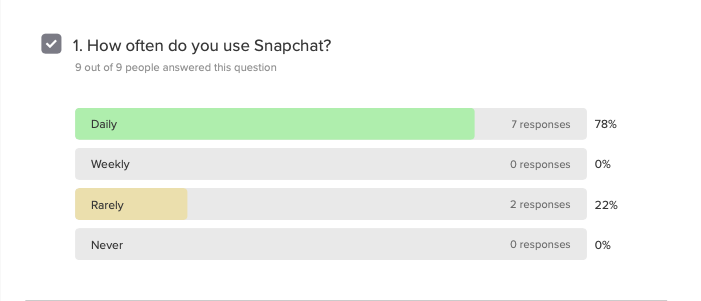
\includegraphics[scale=0.6]{survey figure 1.png}
    \caption{Survey Q1}
    \label{fig:label}
\end{figure}

\begin{figure}[h!]
    \centering
    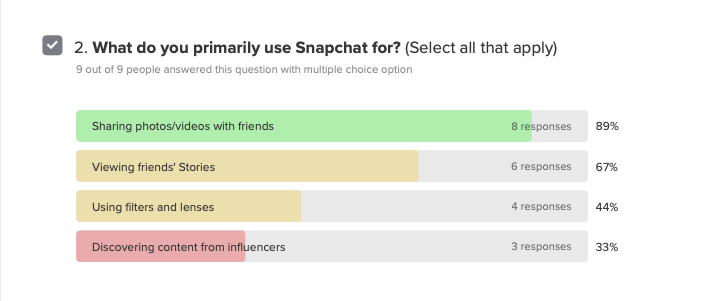
\includegraphics[scale=0.6]{survey figure 2.png}
    \caption{Survey Q2}
    \label{fig:label}
\end{figure}

\begin{figure}[h!]
    \centering
    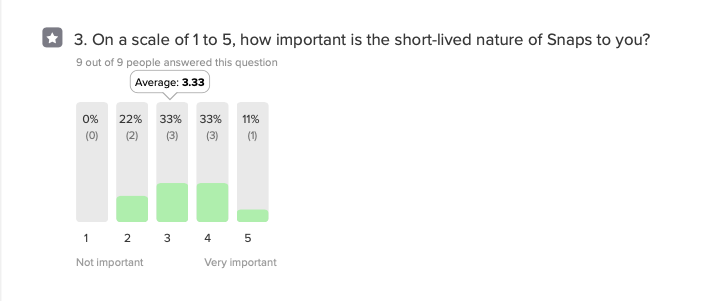
\includegraphics[scale=0.6]{survey figure 3.png}
    \caption{Survey Q3}
    \label{fig:label}
\end{figure}

\newpage
\begin{figure}[h!]
    \centering
    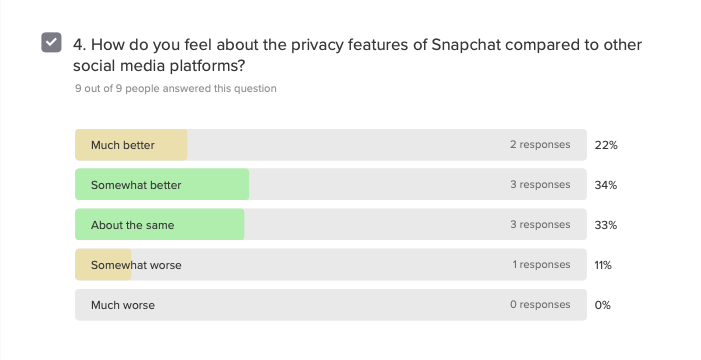
\includegraphics[scale=0.6]{survey figure 4.png}
    \caption{Survey Q4}
    \label{fig:label}
\end{figure}

\begin{figure}[h!]
    \centering
    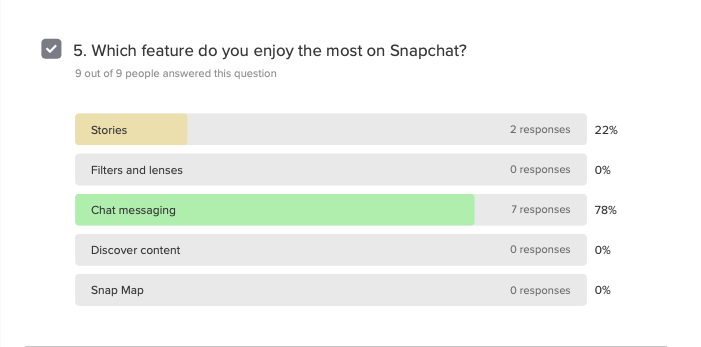
\includegraphics[scale=0.6]{survey figure 5.png}
    \caption{Survey Q5}
    \label{fig:label}
\end{figure}

\begin{figure}[h!]
    \centering
    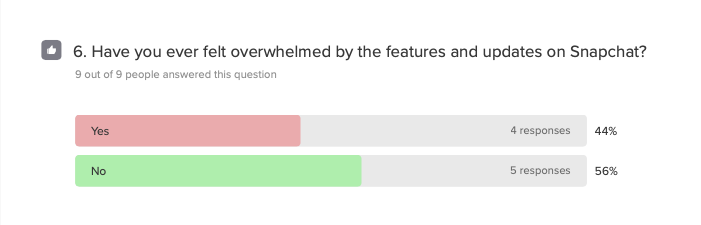
\includegraphics[scale=0.6]{survey figure 6.png}
    \caption{Survey Q6}
    \label{fig:label}
\end{figure}

\newpage
\begin{figure}[h!]
    \centering
    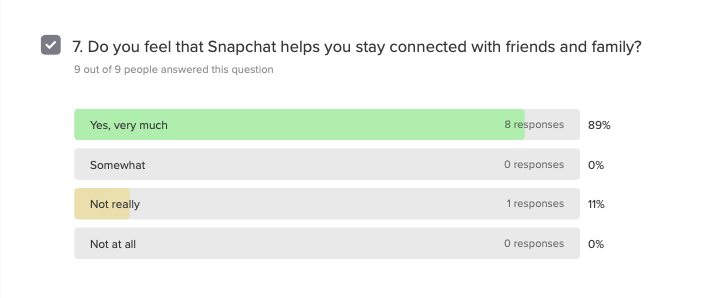
\includegraphics[scale=0.6]{survey figure 7.png}
    \caption{Survey Q7}
    \label{fig:label}
\end{figure}

\begin{figure}[h!]
    \centering
    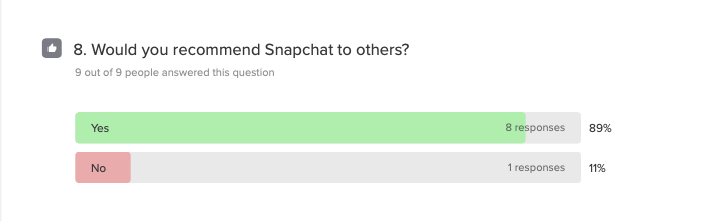
\includegraphics[scale=0.6]{survey figure 8.png}
    \caption{Survey Q8}
    \label{fig:label}
\end{figure}
As shown in figure 1 It is evident that users rely on Snapchat to communicate on a daily basis. With it's many features, users see the app as great way to stay connected with friends and family in fun ways (refer to figure 7).
Snapchat provides users with a platform to share and interact with multimedia content, using features like Stories, filters, and location sharing.





\newpage
\subsection{Existing Programs}

\begin{longtable}{|p{2cm}|p{6cm}|p{6cm}|}
    \hline
    \textbf{Program} & \textbf{TikTok} & \textbf{Instagram} \\
    \hline
    Advantage & 
    • Primarily focused on short-form video content (15 to 60 seconds).\newline
    • Superior video-editing features and creative tools like filters, effects, and music integration.\newline
    • Algorithm-driven, delivering highly tailored content based on user behavior.\newline

    & 
    • Supports multiple content formats (photos, videos, stories, live streams, and Reels). \newline
    • Offers image editing tools and filters for detailed photo posts. \newline
    • Two-factor authentication (2FA) and account protection measures. \\
    \hline
    Disadvantage & 
    • Less suited for static content. \newline
    • Content feed can feel repetitive and highly addictive. 
    & 
    • The app has become complex with too many features, which can be overwhelming. \newline
    • Less focused on discovering content from strangers; primarily a follower-based model.\\
    \hline
    \caption{Existing Programs: Instagram vs TikTok}
    \label{tab:comparison}
\end{longtable}

Snapchat, despite its differences from Instagram and TikTok, addresses some of the disadvantages of each platform in specific ways. Here's how Snapchat can be considered better in certain areas based on the the comparison in Table 1: \newline
-	Compared to Instagrams overwhelming features, Snapchat focuses primarily on temporary content (snaps and stories) with a more straightforward interface. \newline
-	TikTok's Content is permanent unless manually deleted, and it is heavily focused on viral, public content. While Snapchat was built around the idea of disappearing content, giving users more control over their privacy. The content (Snaps and Chats) automatically deletes after viewing or a set period


\newpage
\section{Analysis}

In this section we specify the project requirements for the Snapchat application.
\subsection{Functional Requirements}
\subsubsection{User Requirements}
\begin{enumerate}
    \item The user should be able to register an account and/or log in using email, phone number, or username.
    \item The user should be able to manage their profile: update personal information (name, username, Bitmoji, birthday), and change their profile picture.
    \item The user should be able to send and receive Snaps (photos, videos) and text messages.
    \item The user should be able to use filters, lenses, and other creative tools for Snaps.
    \item The user should be able to manage their friends list: add new friends, remove friends, and block/unblock users.
    \item The user should be able to create and manage stories that are visible to friends or the public.
    \item The user should be able to access and use group chats.
    \item The user should be able to use Discover to explore content from media partners.
    \item The user should be able to make voice and video calls.
    \item The user should be able to access and use the Snap Map to see where their friends are and share their location.
    \item The user should be able to manage privacy settings: control who can send Snaps, view stories, and see their location.
    \item 
\end{enumerate}

\subsubsection{System Requirements}
\begin{enumerate}
    \item The system should handle multiple user sessions and maintain real-time updates (Snaps, stories, messages) without significant delays.
    \item The system should ensure secure communication and transmission of Snaps using encryption.
    \item The system should be able to store and manage large volumes of multimedia content (Snaps, stories) in a temporary fashion (e.g., auto-deleting after viewing or after 24 hours).
    \item The system should support high-quality video and image processing for Snaps, filters, and lenses.
    \item The system should generate notifications for users about new Snaps, chats, friend requests, and updates from Discover.
    \item The user interface should be intuitive, minimalistic, and optimized for mobile devices.
    \item The application should be compatible with major app stores (e.g., Google Play Store, Apple App Store).
\end{enumerate}


\subsection{Non-Functional Requirements}
\begin{enumerate}
    \item Security and Privacy: Ensure end-to-end encryption for all Snaps and messages. Secure user data, especially personal details and location, and prevent unauthorized access.
    \item Availability: The app should be available 24/7 with minimal downtime. Ensure high uptime for critical features like messaging and Snap sending/receiving.
    \item Performance: Ensure that the app operates smoothly across different mobile devices with minimal lag, especially in filters, stories, and Snap processing.
    \item Usability: The app interface should be easy to navigate, with user-friendly icons and features, ensuring users can quickly access Snaps, stories, and the camera.
    \item Scalability: The system should be able to handle increasing numbers of users without a decline in performance, especially during peak hours.
    \item Reliability: The app should provide consistent performance, with minimal crashes or errors during Snap creation, viewing, or messaging.
\end{enumerate}
 
In conclusion, we have detailed the essential functional and non-functional requirements for the Snapchat application. These requirements ensure the app delivers a secure, user-friendly, and high-performing experience, leading to a successful development and operation.

\newpage
\section{Design}

In this section we will represent the Snapchat architecture system in the folloing points: Application user interface - UI, Database and Data Model, and finally the Programming Languages.
\subsection{Architecture System}
\subsubsection{User Interface}
Snapchat’s user interface - UI is minimalistic and intuitive, with the camera screen serving as the core, allowing users to quickly take photos or videos. Navigation through the app is seamless, thanks to buttons placed at the bottom of the screen to switch between features like chats and stories. Snapchat is known for its use of augmented reality - AR lenses and temporary messaging, which enhance the user experience. \newline

\begin{figure}[h]
    \begin{minipage}{0.15\textwidth} 
        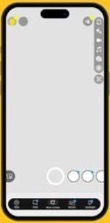
\includegraphics[width=\linewidth]{Home.jpg} 
        \caption{Home Screen UI}
        \label{fig:homescreen}
    \end{minipage}
    \begin{minipage}{0.80\textwidth} 
        The camera functionality is at the core of the home screen, allowing users to take photos and record videos with various creative tools and filters. The navigation buttons on the home screen enable users to access different sections of the app easily. strategically placed at the bottom of the screen, provide quick and seamless navigation between the camera, chat, and discover pages.\newline
    \end{minipage}
\end{figure}

\begin{figure}[h]
    \begin{minipage}{0.15\textwidth} 
        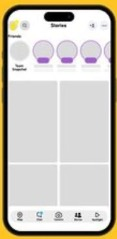
\includegraphics[width=\linewidth]{discover.jpg} 
        \caption{Discover Page UI}
        \label{fig:discover page}
    \end{minipage}
    \begin{minipage}{0.80\textwidth} 
        The discover page is where users can explore a wide range of content from various publishers, influencers, and brands. The discover page showcases a curated selection of personalized recommendations based on the user’s interests and preferences. This personalized approach to content discovery keeps users engaged and ensures they are always presented with content that resonates with them. \newline
    \end{minipage}
\end{figure}

\newpage
\begin{figure}[h]
    \begin{minipage}{0.15\textwidth} 
        
\includegraphics[width=\linewidth]{chatlist.jpg}
        \caption{Chat List UI}
        \label{fig:image1}
    \end{minipage}
    \begin{minipage}{0.15\textwidth} 
        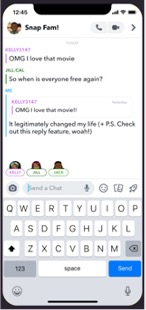
\includegraphics[width=\linewidth]{chat.jpg}
        \caption{Chat UI}
        \label{fig:image2}
    \end{minipage}
    \begin{minipage}{0.15\textwidth} 
        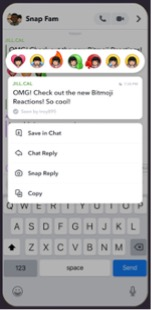
\includegraphics[width=\linewidth]{chat.interaction.jpg} 
        \caption{Chat Interaction UI}
        \label{fig:image3}
    \end{minipage}
\end{figure}
The messaging features, including text, voice, and video chat, are seamlessly integrated into the app’s UI. Users can easily send messages, photos, and videos to their friends, creating a dynamic and interactive communication experience. \newline

\begin{figure}[h]
    \begin{minipage}{0.15\textwidth} 
        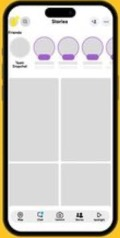
\includegraphics[width=\linewidth]{stories.jpg} 
        \caption{Stories UI}
        \label{fig:stories}
    \end{minipage}
    \begin{minipage}{0.80\textwidth} 
        The UI design for stories enables users to share their moments in a chronological narrative, creating a captivating storytelling experience. Users can swipe through stories effortlessly, making it easy to navigate through continuous stream of content from their friends and favorite accounts.
    \end{minipage}
\end{figure}

\begin{figure}[h]
    \centering
    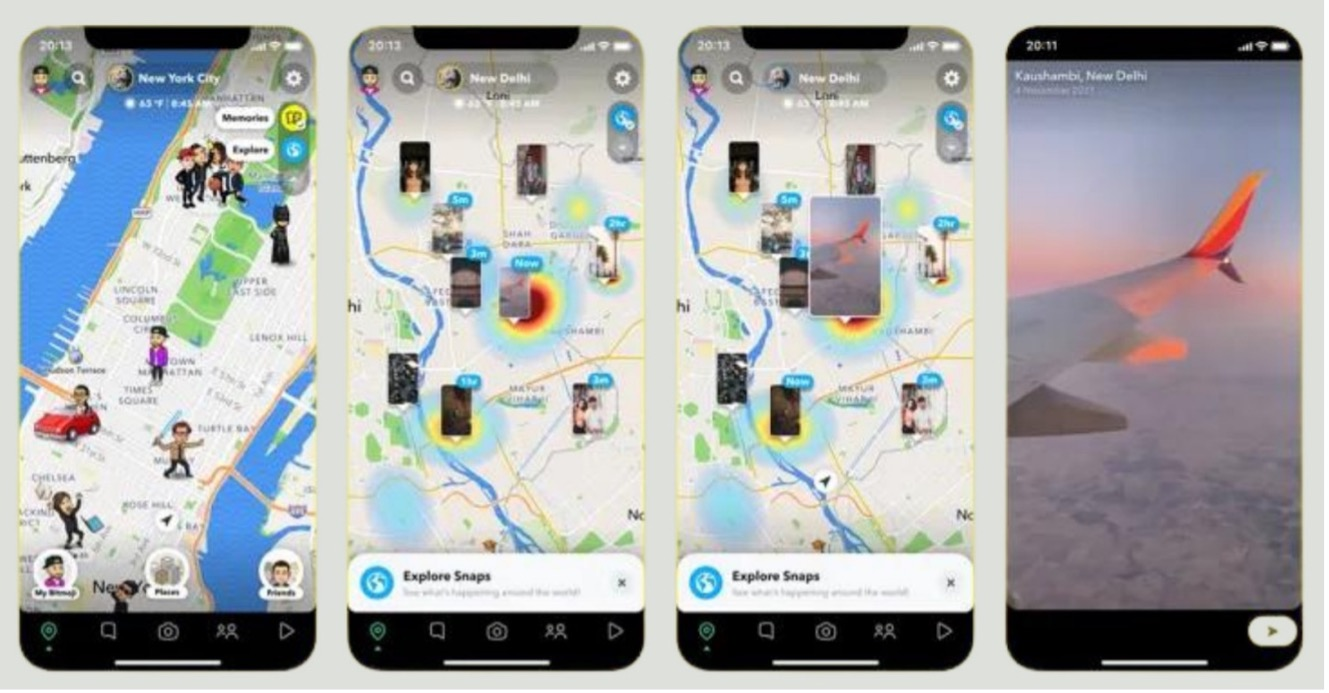
\includegraphics[width=0.5\linewidth]{snapMap.jpg}
    \caption{Snap Map UI}
    \label{fig:snap map}
\end{figure}

Snapchat’s Snap Map allows users to see where their friends are on a real-time map. fostering a sense of connection and shared experiences. However, Users have full control over their location visibility, choosing who can see them and even creating “ghost mode” for complete invisibility. \newline

\newpage
\subsubsection{Data Models}
Sign up/login process activity diagram:
\begin{figure}[h]
    \centering
    \includegraphics[width=0.75\linewidth]{signup:login.drawio.png}
    \caption{Sign up/login process activity diagram}
    \label{fig:activity diagram}
\end{figure}

\newpage
Stories function activity diagram:
\begin{figure}[H]
    \centering
    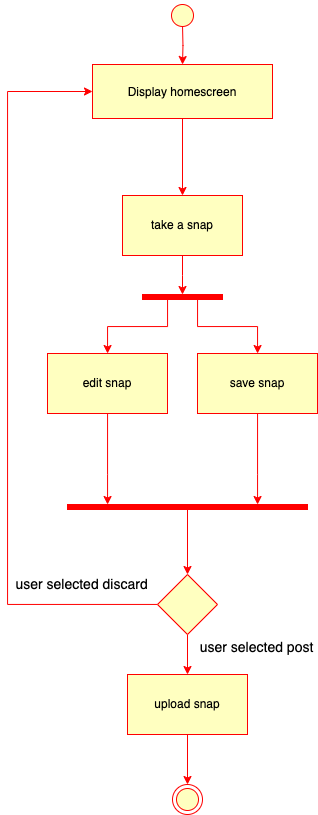
\includegraphics[width=0.50\linewidth]{stories.drawio.png}
    \caption{Stories function activity diagram:}
    \label{fig:activity diagram}
\end{figure}

\newpage
\subsubsection{Database}
Originally, Sanapchat's database operated on a monolithic architecture but transitioned to microservices to improve scalability and performance. Key components of its data infrastructure now include Amazon DynamoDB, a NoSQL database known for its ability to provide low-latency performance and handle millions of queries per second. This technology powers critical Snapchat services, such as messaging and the "friend graph" used for managing user connections. The shift to DynamoDB also enabled Snapchat to regionalize its database, reducing latency for users worldwide. \newline


There is no way of  knowing how Snapchat's database actually looks like. but if we were to illustrate some parts of it based on user experience it would look something like this: 
\newline
\newline
\textbf{Users Information:}
\begin{figure}[H]
    \centering
    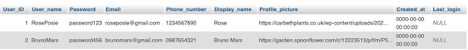
\includegraphics[width=1\linewidth]{Picture1.png}
    \caption{Snapchat Database: User Information Table Example}
    \label{fig:User Information Table Example}
\end{figure}
\textbf{Snaps Log:}
\begin{figure}[H]
    \centering
    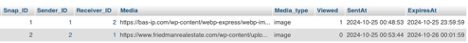
\includegraphics[width=1\linewidth]{Picture2.png}
    \caption{Snapchat Database: Snaps Log Table Example}
    \label{fig:Snaps Log Table Example}
\end{figure}

Based on the login/sign in process data, the Users table shown in figure 11 Stores data like : user ID, username, password, email, phonenumber, display name and profile picture for every user. While the Snaps table in figure 12 is derived from the Chat "Snaps" process. It stores data like: Sender ID (referensing the User ID in the Users table), Receiver ID (referensing the User ID in the Users table), the media sent, the sent media's type (as Snapchat allows sharing of several media types through chat), snap viewing state, the timestapm of the sent snap, as well as the timestamp of it's expiration (as snaps disappear after 24 hours).

\subsubsection{Programming Languages}
\begin{enumerate}
    \item Python:
 Used for server development and data processing. Python is ideal for writing scripts and managing data
    \item Java:
Used for developing Android applications. Java is a powerful language and is suitable for mobile applications
    \item Objective-C and Swift:
Used for developing iOS applications. Objective-C was the primary language, but Swift has become more popular due to its ease of use and efficiency.
    \item JavaScript:
Used for developing user interfaces and web-specific features. JavaScript is essential for dynamic interaction on the web and mobile applications.
    \item C++:
Used for performing complex tasks such as image and video processing. C++ provides high performance, making it ideal for resource-intensive operations.
\end{enumerate}

\newpage
\section{References}
\begin{thebibliography}{9}
\bibitem{medium}
Realize, N. (2023, May 24). \emph{The Power of Online Communication: Understanding the Importance of Effective Interaction in the Digital Era}. Medium. Retrieved from \url{https://medium.com/@nowrealize/the-power-of-online-communication-understanding-the-importance-of-effective-interaction-in-the-94f4e7ed55df}

\bibitem{litcommerce}
Nguyen, L. (2024, September 17). \emph{TikTok vs Instagram: 9 Key Differences}. Retrieved from \url{https://litcommerce.com/blog/tiktok-vs-instagram-comparison/}

\bibitem{buffer}
Buffer. (n.d.). \emph{Instagram and Snapchat: A Full Comparison}. Retrieved from \url{https://buffer.com/resources/instagram-vs-snapchat/}

\bibitem{brafton}
King, D. (2024, July 19). \emph{TikTok vs Snapchat: Differences, Pros and Cons (Infographic)}. Brafton. Retrieved from \url{https://www.brafton.com/blog/social-media/tiktok-vs-snapchat/}

\bibitem{rawstudio}
Estefani, J. N. A. (2024, February 16). \emph{Unveiling The Magic: A Deep Dive Into Snapchat's UI Design Strategies}. Raw.Studio. Retrieved from \url{https://raw.studio/blog/unveiling-the-magic-a-deep-dive-into-snapchats-ui-design-strategies/}

\bibitem{freepik}
Premium Vector | Snapchat app Screen Intrace Mockup Snapchat mockup iPhone layout Social media for iPhone Template interface Makte temleit User interface. (2023, June 21). Freepik. Retrieved from \url{https://www.freepik.com/premium-vector/snapchat-app-screen-intrace-mockup-snapchat-mockup-iphone-layout-social-media-iphone-template-interface-makte-temleit-user-interface_49416215.htm}

\bibitem{hashdork}
Jay. (2024, May 27). \emph{Snapchat System Design \& Architecture}. HashDork. Retrieved from \url{https://hashdork.com/snapchat-system-design-architecture/}

\bibitem{aws}
Reduce Median Latency by 20\% Using Amazon DynamoDB | Snap Case Study | AWS. (n.d.). Amazon Web Services, Inc. Retrieved from \url{https://aws.amazon.com/ar/solutions/case-studies/snap-dynamodb/}

\bibitem{apptunix}
Nalini. (2024, June 6). \emph{How Much Does it Cost to Build an App like Snapchat [Roadmap + Costing]}. Apptunix Blog. Retrieved from \url{https://www.apptunix.com/blog/the-complete-guide-to-snapchat-like-app-development-cost-for-2024/}
\end{thebibliography}


\end{document}